\newpage
\section{Теорема Коши для односвязных и многосвязных областей}
\textbf{Теорема 1 (Коши для односвязной области)}\\
Если $D \subset \mathbb{C}$ -- односвязная область, $f \in H(D)$ ($f$ голоморфна), $\gamma \subset D$ -- замкнутая кривая, то \(\int_{\gamma} f\, dz\) $= 0$.


\begin{proof}
    \ \\
    Для случая, когда $f'(z)$ непрерывная в $D$:\\
    $z=x+iy$; $f(z)=u(x,y)+iv(x,y)$\\
    $I = \int\limits_{\gamma}fdz = \int\limits_{\alpha}^{\beta}f(z(t))z'(t)dt = \int[u(zx(t),y(t))+iv(x(t), y(t))]\cdot [x'(t)+it'(t)]dt = \int\limits_{\alpha}^{\beta}[u\cdot x'-v\cdot y')+i(uy'+vx')]dt=\int\limits_{\alpha}^{\beta}(ux'-vy')dt+i\int\limits_{\alpha}^{\beta}(uy'+vx')dt = \int\limits_{\gamma}udx-vdy +i\int\limits_{\gamma}udy+vdx=$
    Разрежем $\gamma$ на простые контуры $\gamma_i$:\\
    $\gamma=\bigcup\limits_{j=1}^{k}\gamma_j$, $G_j$ -- область внутри $\gamma_j$\\
    $I = \sum_{j=1}^k \left[ \oint\limits_{\gamma_j}u\,dx-v\,dy+i\oint\limits_{\gamma_j}v\,dx+u\,dy \right] =$\\
    $= \sum_j \left[ \iint\limits_{G_j}\left(-\frac{\partial v}{\partial x}-\frac{\partial u}{\partial y} \right)dx\,dy + i\iint\limits_{G_j}\left(\frac{\partial u}{\partial x}-\frac{\partial v}{\partial y} \right)dx\,dy \right] = 0$
\end{proof}


\textbf{Теорема 2 (Коши для многосвязной области)}\\
\begin{figure}[!ht]
\begin{center}
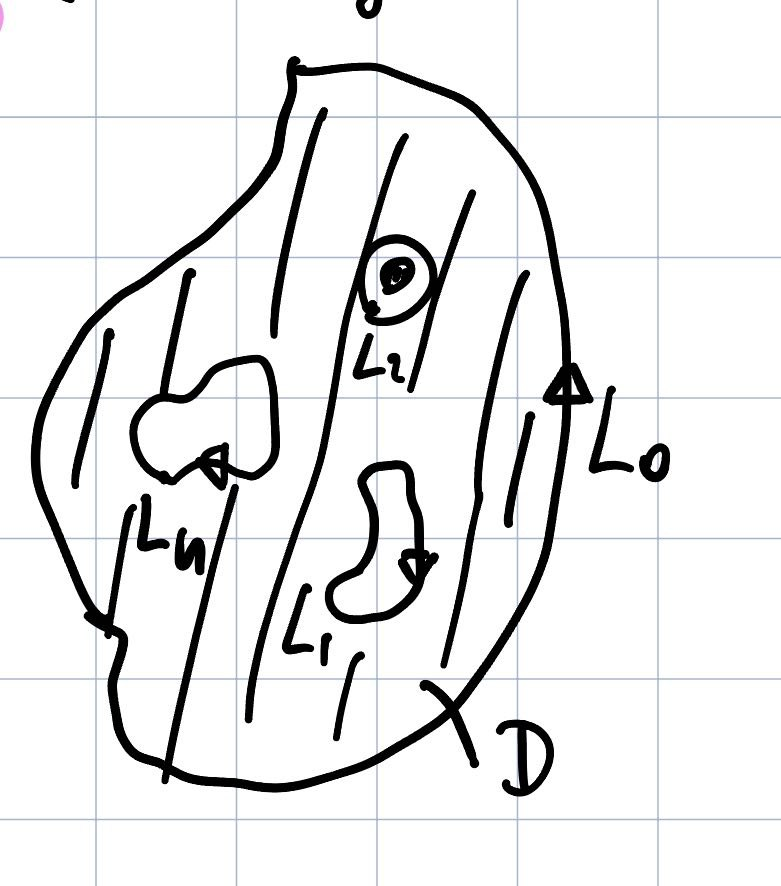
\includegraphics[scale=0.2]{answers/img/pic3.jpg}
\end{center}
\end{figure}\\
Пусть многосвязная область $D$ ограничена внешним контуром $L_0$ и внутренними контурами $L_1$, ..., $L_n$, контуры $L_1$, ..., $L_n$ -- кусочно-гладкие, $f \in H(D \cup L_0 \cup L_1 \cup$ ... $\cup L_n)$.\\
Тогда \(\int_L f\, dz\) $= 0$, где $L = L_0 \cup L_1 \cup$ ... $\cup L_n$, обход $L_0$ -- против часовой стрелки, $L_1$, ..., $L_n$ -- по часовой стрелке.\\
\textbf{Замечание.} \(\oint_{L_0} f\, dz\) 
$= \sum_{i = 1}^{n}$\(\oint_{L_i} f\, dz\), где обход $L_0$, $L_1$, ..., $L_n$ против часовой стрелки.


\begin{proof}
    \ \\
    С помощью разрезов $\gamma_1, ..., \gamma_n$ получим односвязную область $D^*$. Тогда $D=D^*\cup\gamma_1\cup...\cup\gamma_n$.\\
    Так как $D^*$--односвязная, то $0=\int\limits_{D^*}fdz = $\\
    Граница $D^* = L_0\cup\gamma_1\cup-\gamma_1\cup L_1 \cup...\cup\gamma_n\cup-\gamma_n\cup L_n$.\\
    Тогда из аддитивности и ориентированности:\\
    $=\int\limits_{L_0}fdz+\sum_{i=1}^n\left[ \int\limits_{\gamma_i}fdz+\int\limits_{-\gamma_i}fdz+\int\limits_{L_i}fdz \right] = \int\limits_{L}fdz=0$
\end{proof}
